% Author: Dr. Matthias Jung
% Year: 2022
\begin{circuitikz}[background rectangle/.style={fill=white}, show background rectangle]
        \node(0,0) {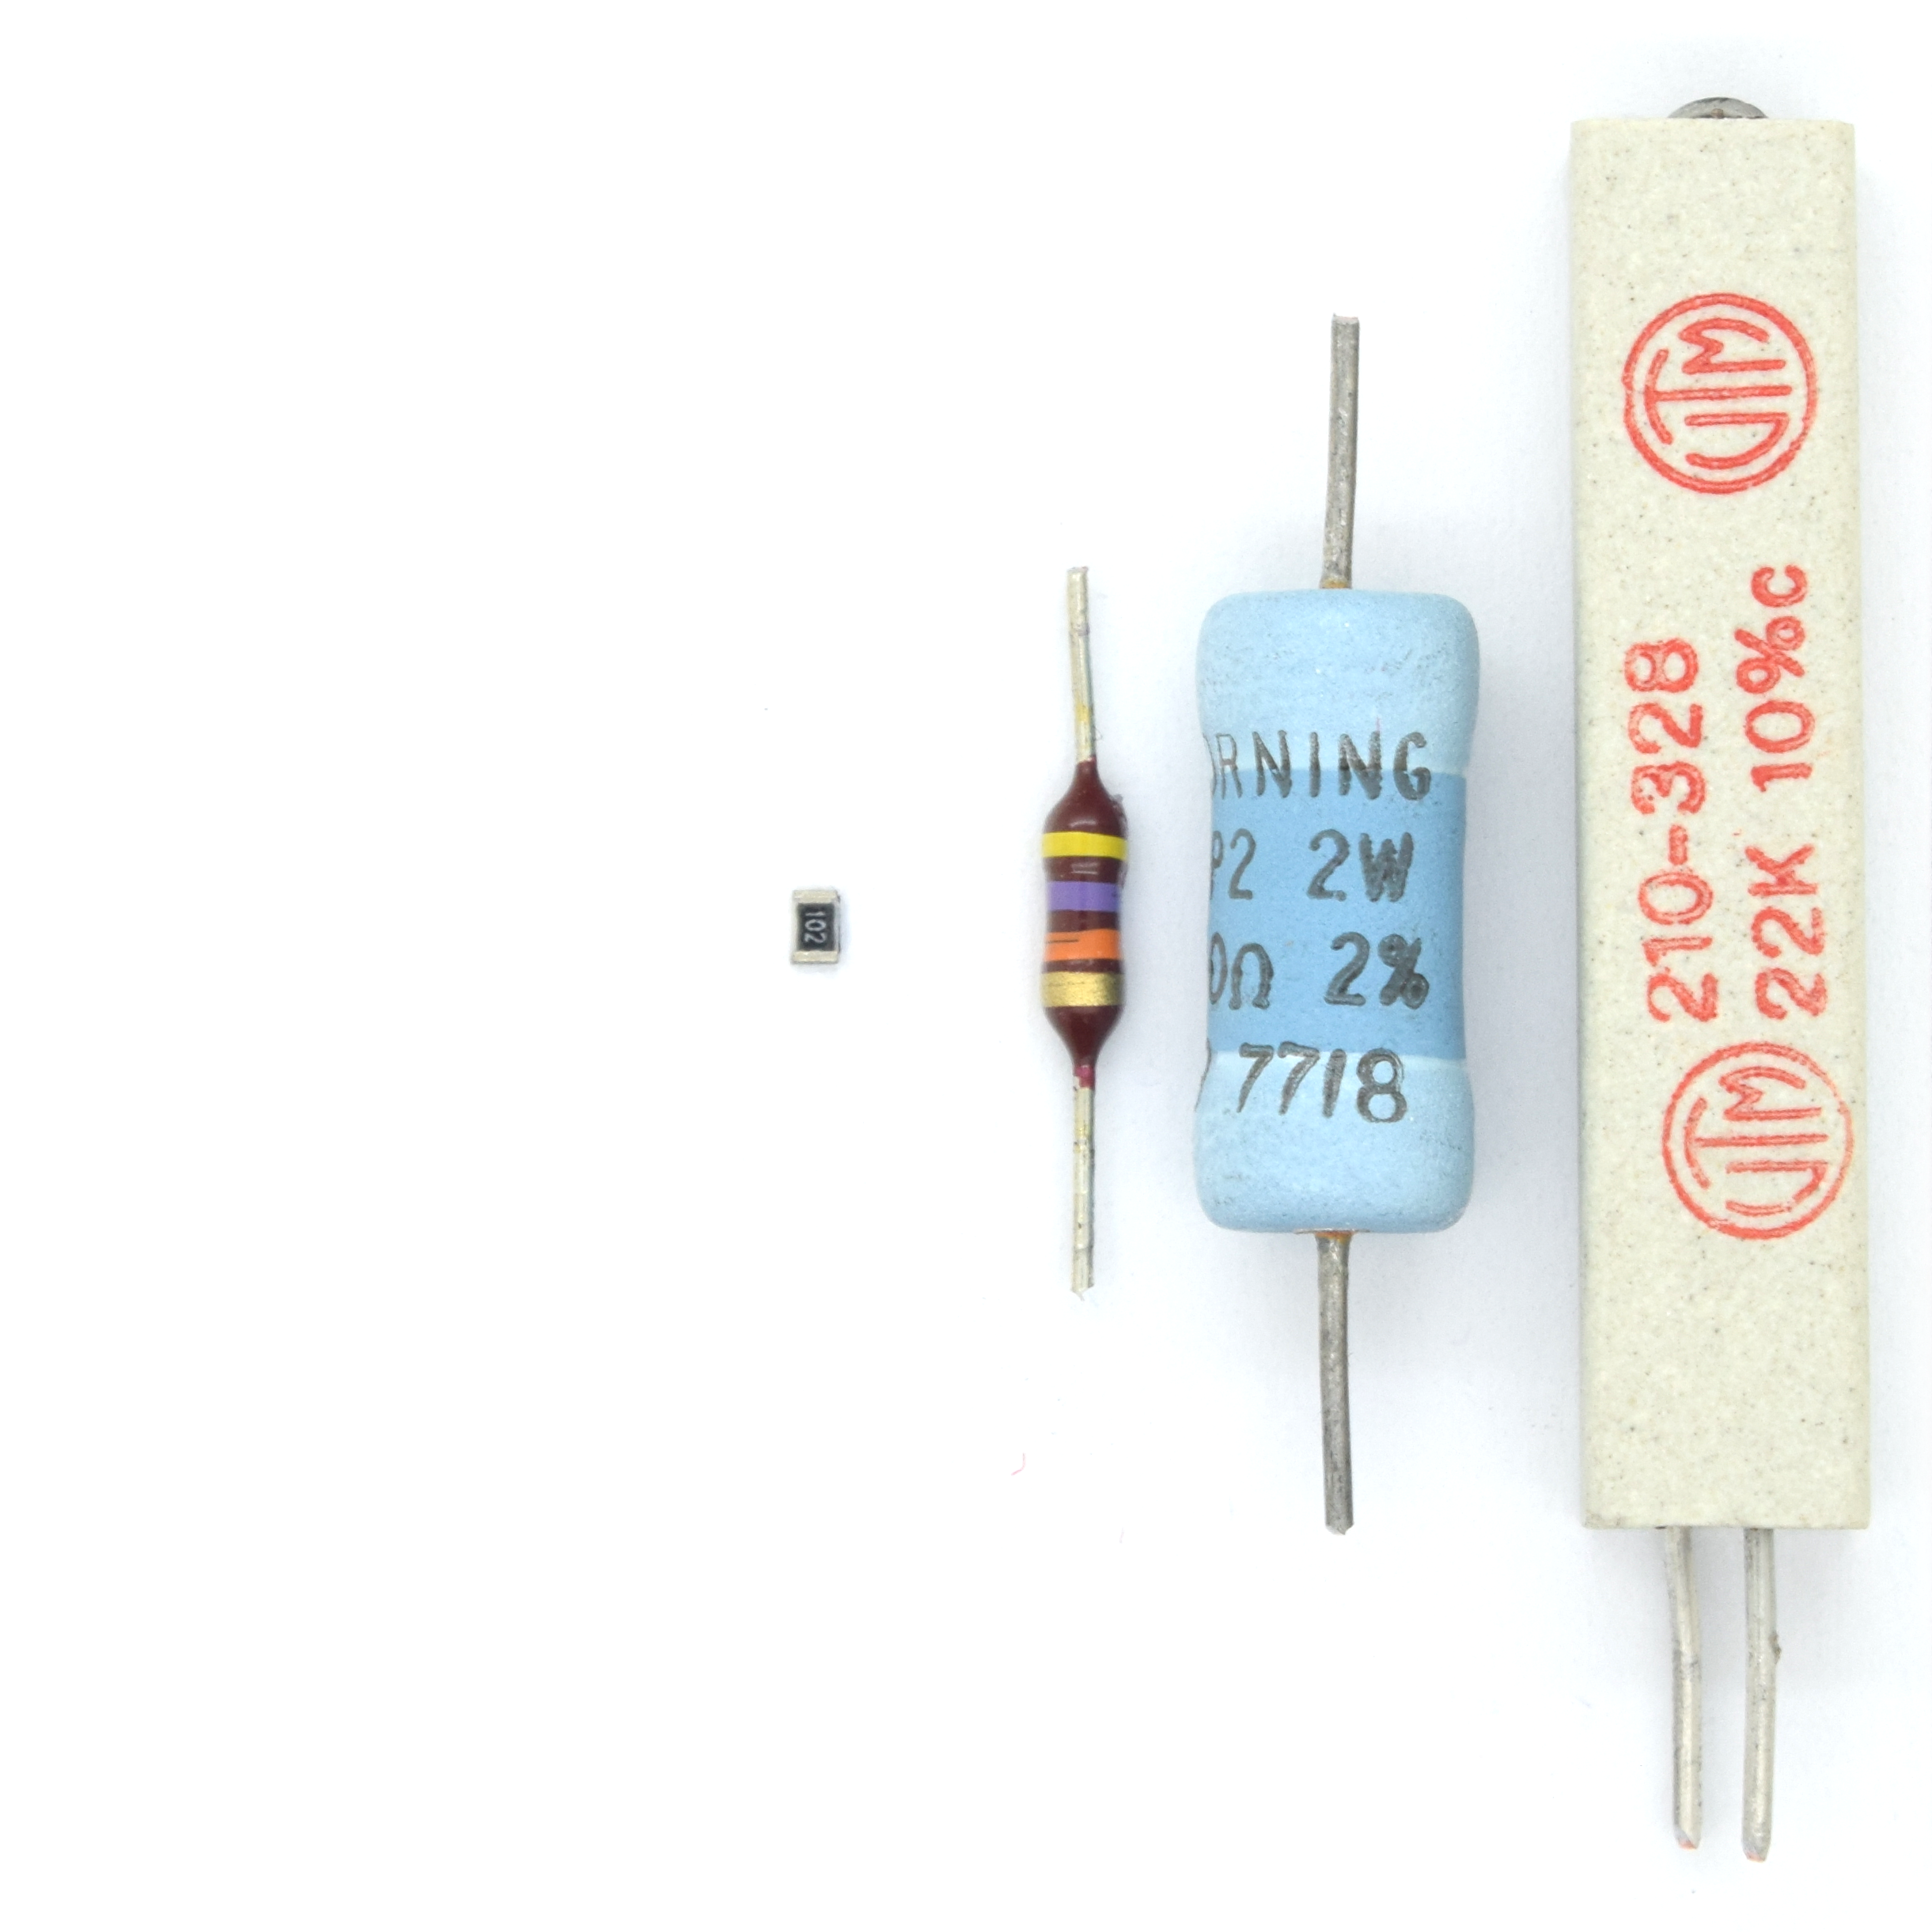
\includegraphics[width=200pt]{foto/1}};

        %Widerstand:
        \draw(-3.0,1) to [R, european,l={$R$}] ++(0,-2);
    
        % SMD:
        \draw(-0.5,  -0.5) node {\small\qty{125}{\milli\watt}};
        \draw(-0.5,  0.75) node {\small\qty{1}{\kilo\ohm}};
        \draw( 0.4,  -1.5) node {\small\qty{250}{\milli\watt}};
        \draw( 0.4,  1.75) node {\small\qty{47}{\kilo\ohm}};
        \draw( 1.3,  -2.5) node {\small\qty{2}{\watt}};
        \draw( 1.3,  2.75) node {\small\qty{620}{\kilo\ohm}};
        \draw( 2.7, -3.75) node {\small\qty{9}{\watt}};
        \draw( 2.7, +3.75) node {\small\qty{22}{\kilo\ohm}};
        
        \draw(-0.5, 0.5) node {};
    
        % Pfeile:
        \draw[>=triangle 60, <->] (-2.0,0.675) coordinate(c1) -- ++(0,-1.35) coordinate(c2);
        \draw(c1) -- ++( 0.25,0);
        \draw(c1) -- ++(-0.25,0);
        \draw(c2) -- ++( 0.25,0);
        \draw(c2) -- ++(-0.25,0);
    
        % Text:
        \draw (c1) ++ (0,0.25) node {\qty{1}{\centi\meter}};
\end{circuitikz}